\section{Del 1: Turingmaskin}
\paragraph{Inledning}    
Uppgiften går ut på att skapa och analyzera en turingmaskin som efter antal a:n i input lägger till inversen av en sträng med 0:or och 1:or till höger, startandes med 0 vilket ger 0 -> 01 -> 0110 osv.

\paragraph{Beskrivning av turingmaskinen}
Följande algoritm utvecklades för att lösa problemet.
\begin{verbatim}
1. gå höger tills _, ersätt _ med 0 
    1.1 gå vänster tills _, gå 3

2. gå vänster tills _
3. gå ett steg höger, om ej a, avsluta 
4. om a, ersätt a med _ 
    4.1 gå höger tills 0 eller 1, om _ gå 4.2 
        4.1.1a om 1, ersätt med y   
           4.1.1a.1 gå höger tills _, ersätt med x, gå 4.1.2  
        4.1.1b om 0, ersätt med x 
        4.1.1b.1 gå höger tills _, ersätt med y, gå 4.1.2 

        4.1.2 gå vänster tills _ eller a, gå 4.1  
    
    4.2 gå vänster tills _ eller a, ersätt x med 0 och y med 1 på vägen 
    4.3 gå 2
\end{verbatim}
För tillståndsövergångar hos turingmaskinen se [4] Bilagor.
\newpage
\paragraph{Tidskomplexitet av algoritm}

\begin{center}
    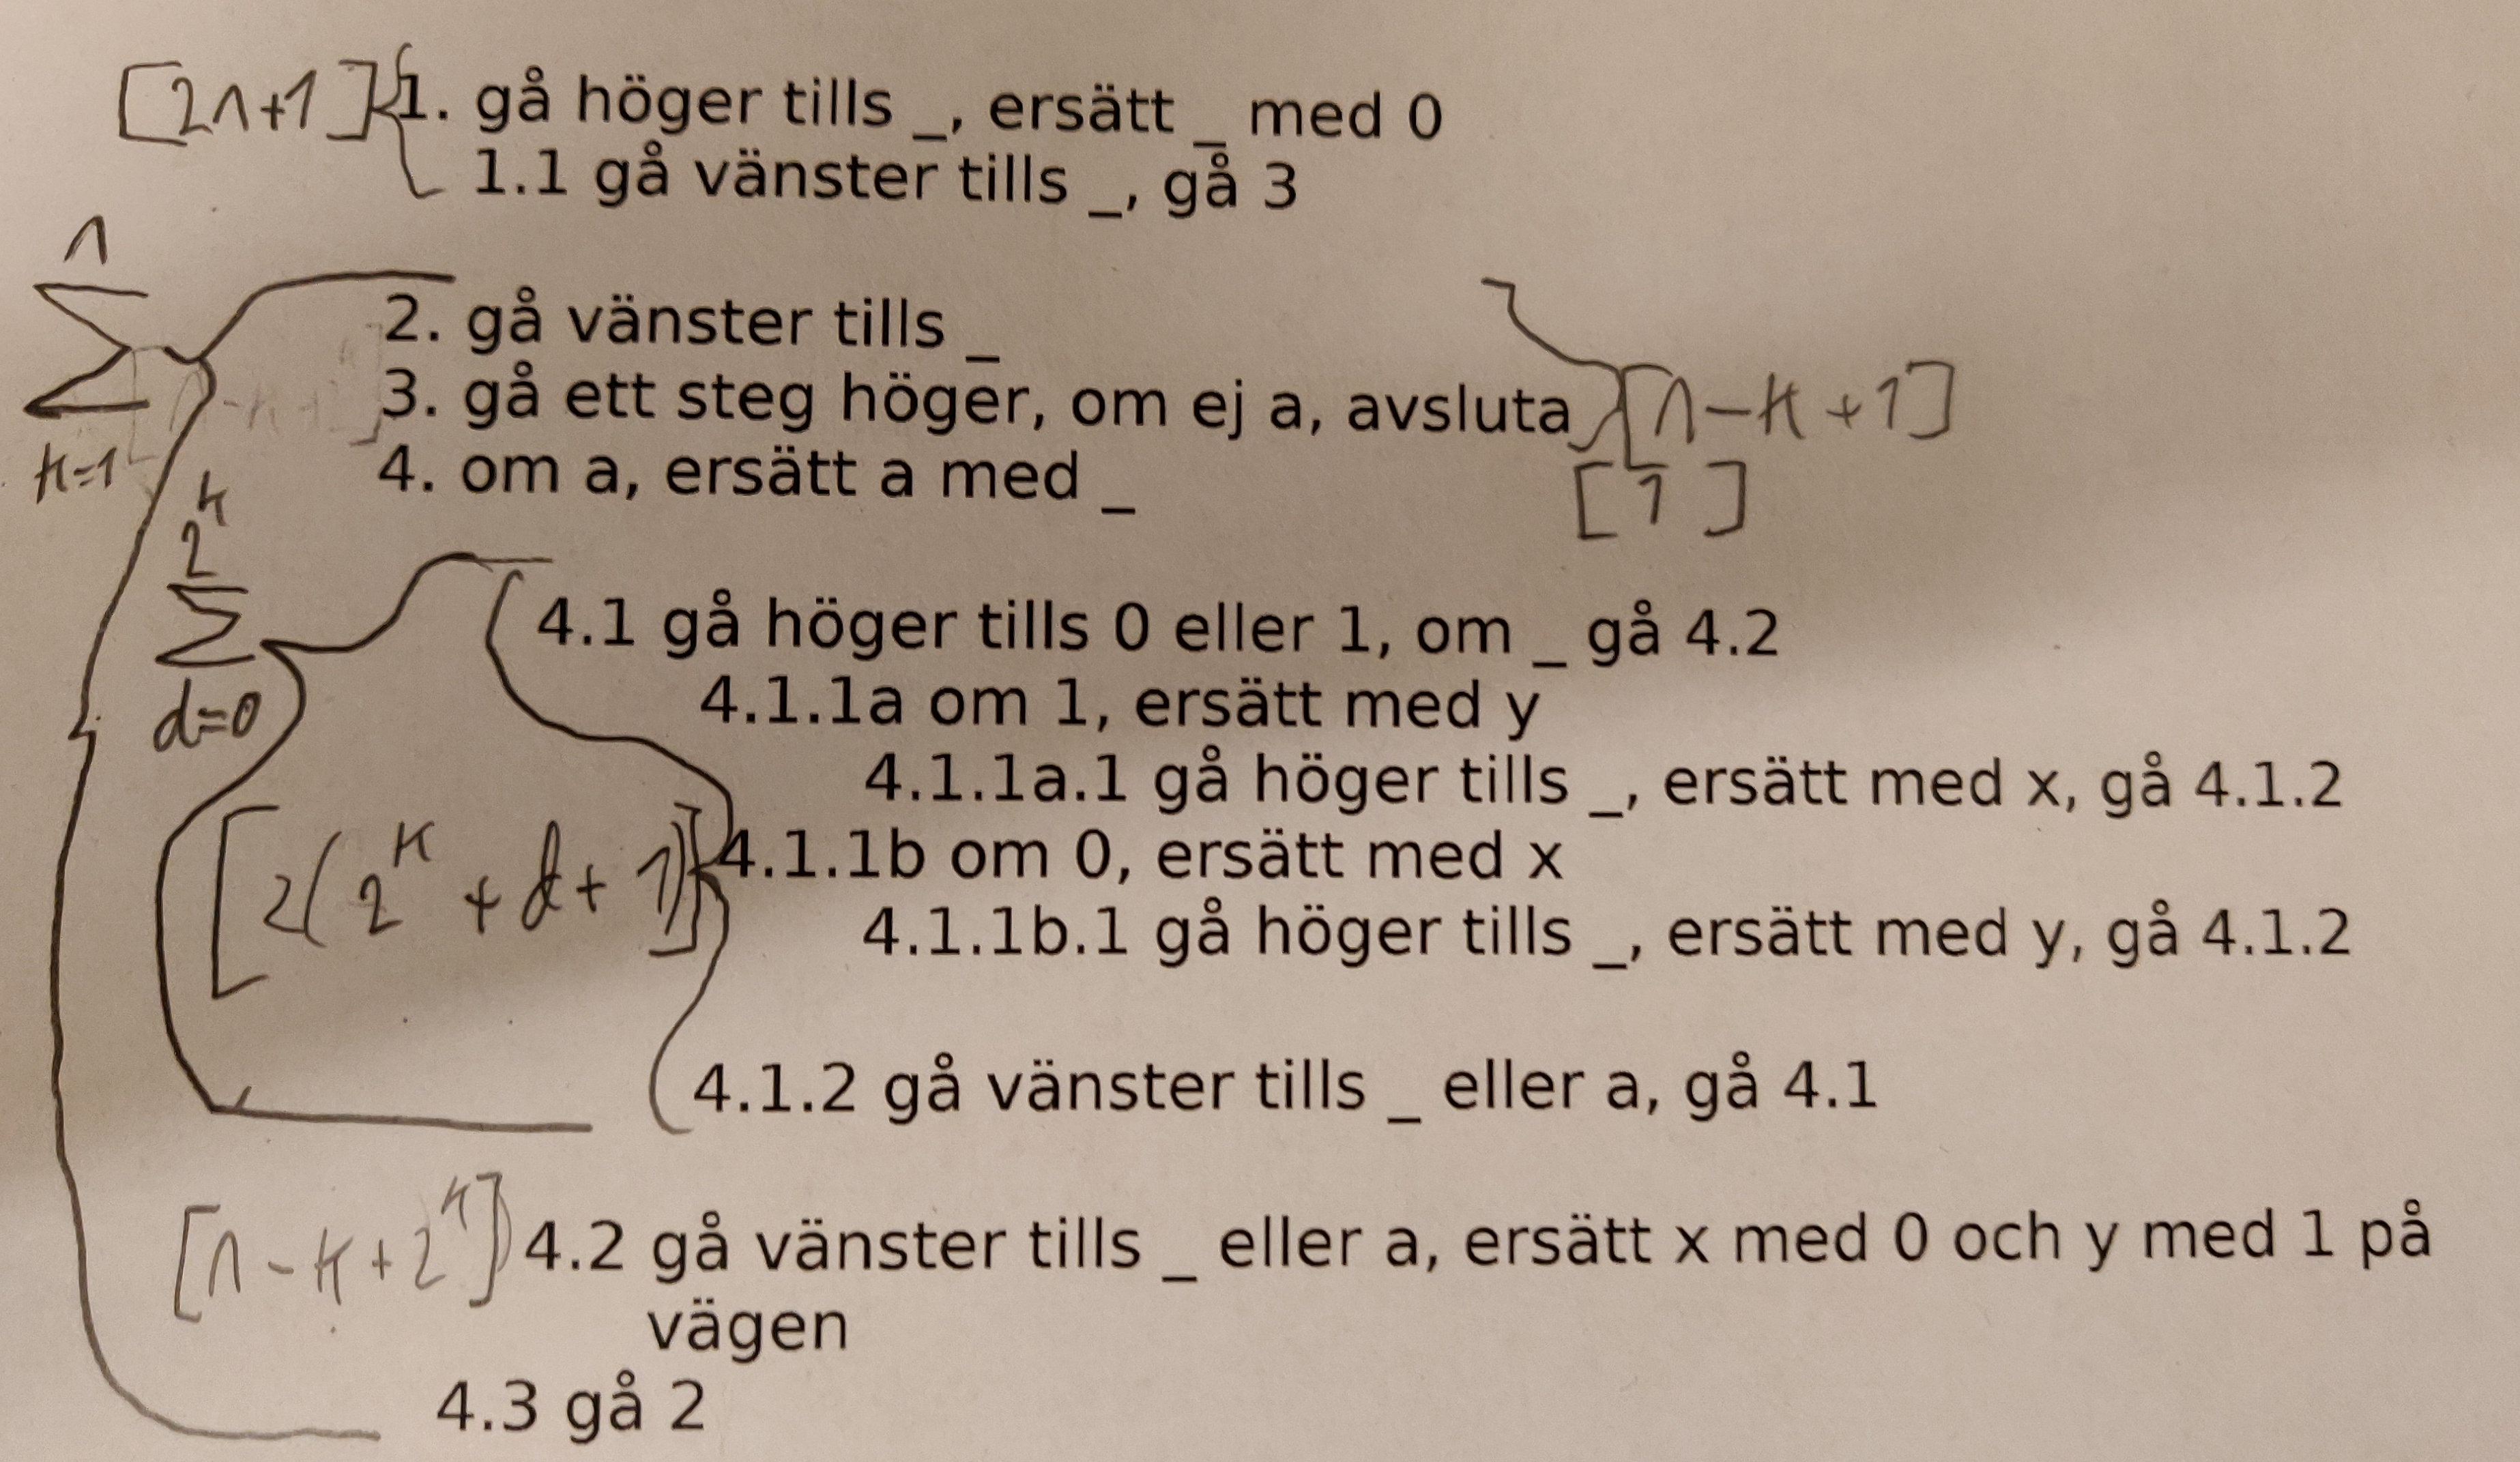
\includegraphics[width=\linewidth]{bilder/komplexitet_analys.jpg}
    \captionof{figure}{Analys av komplexitet per del}
\end{center}

\begin{center}
    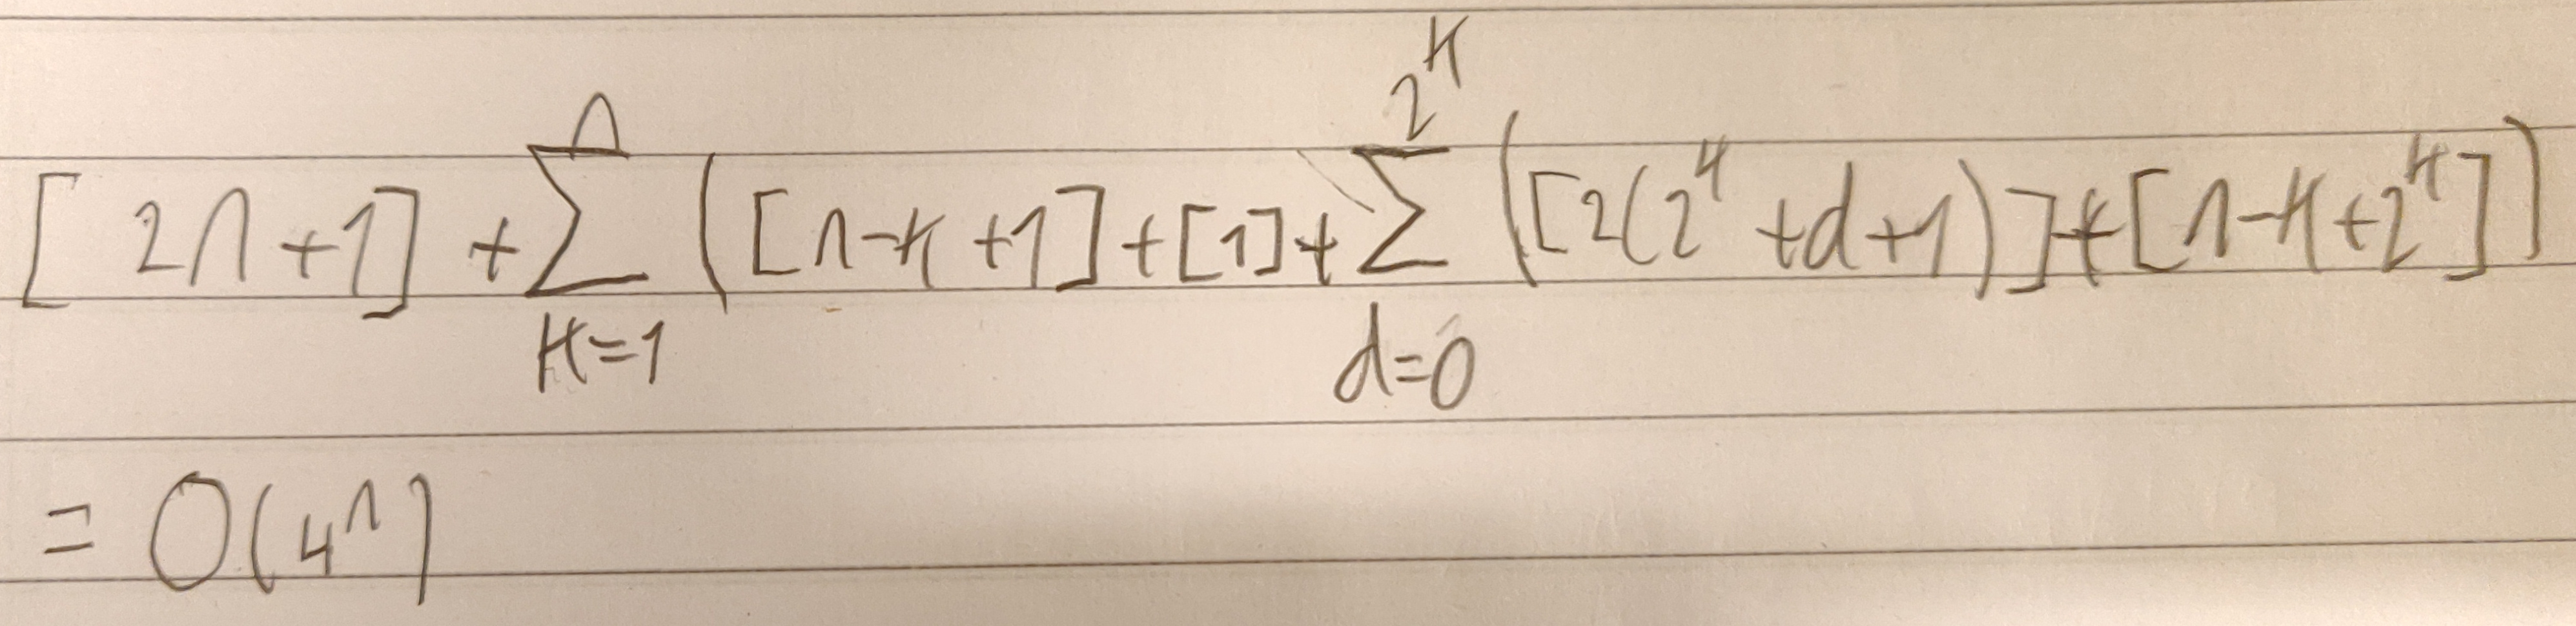
\includegraphics[width=\linewidth]{bilder/komplexitet_utrakning.jpg}
    \captionof{figure}{Uträkning av komplexiteten i O()}
\end{center}
Ur analysen framkommer det att algoritmen har tidskomplexiteten O($4^n$)

Tidskomplexiteten ritades på en linje och jämfördes med flertal datapunkter från när maskinen kördes i simulatorn för att analysera hur korrekt komplexiteten var. 
\begin{center}
    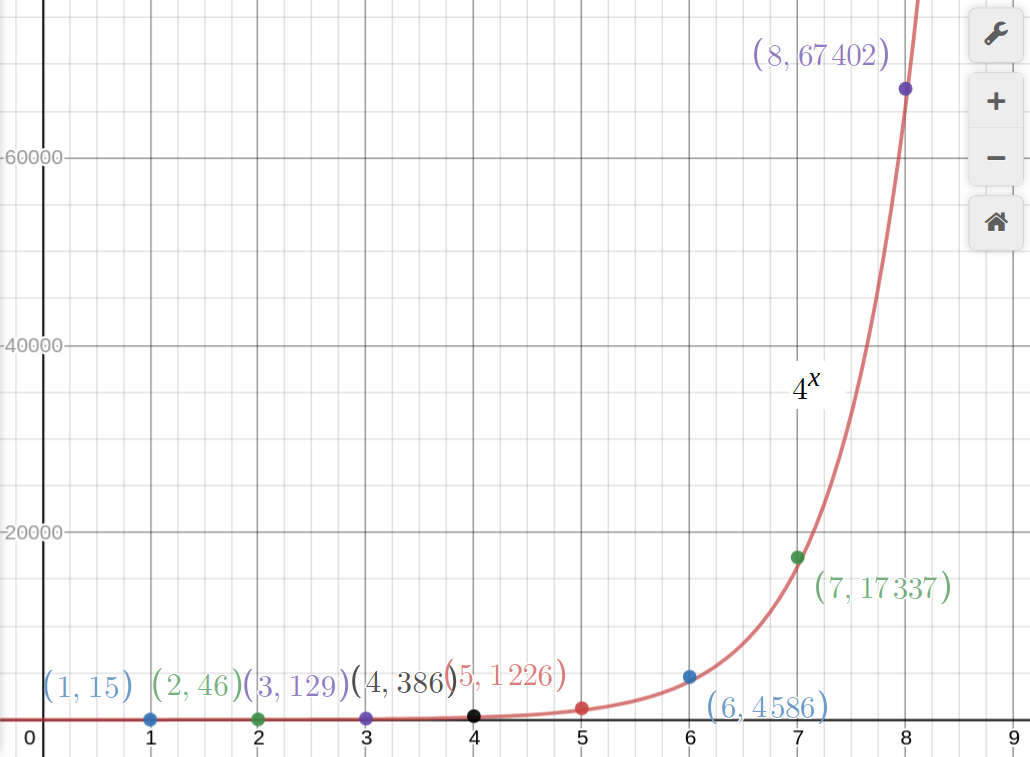
\includegraphics[width=\linewidth]{bilder/graf.png}
    \captionof{figure}{Graf som jämför datapunkter och den uträknade tidskomplexiteten. Y-axeln står för antalet steg och x-axeln för antalet a:n i indatan.}
\end{center}
Av grafen kan det bestämmas att O($4^n$) är den korrekta tidskomplexiteten för algoritmen. 
\newpage
